\documentclass[9pt,aspectratio=43,mathserif,table]{beamer} 
%设置为 Beamer 文档类型,设置字体为 10pt,长宽比为16:9,数学字体为 serif 风格
\batchmode

\usepackage{graphicx}
\usepackage{animate}
\usepackage{hyperref}

%导入一些用到的宏包
\usepackage{amsmath,bm,amsfonts,amssymb,enumerate,epsfig,bbm,calc,color,ifthen,capt-of,multimedia,hyperref}
\usepackage{xeCJK} %导入中文包
\setCJKmainfont{SimSun} %字体采用黑体  Microsoft YaHei

% \usetheme{Marburg} %主题
% \usecolortheme{sustech} %主题颜色
\usetheme{metropolis} %主题
% \usetheme{Montpellier}
\usecolortheme{default} %主题颜色

\usepackage[ruled,linesnumbered]{algorithm2e}

\usepackage{fancybox}
\usepackage{xcolor}
\usepackage{times}

\usepackage{listings}

\usepackage{booktabs}
\usepackage{colortbl}

\usepackage{setspace}

% \usepackage{minted}
% \usemintedstyle{emacs}

\newcommand{\Console}{Console}
\lstset{ %
  % backgroundcolor=\color{white},   % choose the background color
  basicstyle=\footnotesize\rmfamily,     % size of fonts used for the code
  columns=fullflexible,
  breaklines=true,                 % automatic line breaking only at whitespace
  captionpos=b,                    % sets the caption-position to bottom
  tabsize=4,
  commentstyle=\color{mygreen},    % comment style
  escapeinside={\%*}{*)},          % if you want to add LaTeX within your code
  keywordstyle=\color{blue},       % keyword style
  stringstyle=\color{mymauve}\ttfamily,     % string literal style
  numbers=left, 
  % numberstyle=\tiny\color{mygray},
  frame=left,
  rulesepcolor=\color{red!20!green!20!blue!20},
  % identifierstyle=\color{red},
  language=c++,
  morekeywords={alignas,continute,friend,register,true,alignof,decltype,goto,
  reinterpret_cast,try,asm,defult,if,return,typedef,auto,delete,inline,short,
  typeid,bool,do,int,signed,typename,break,double,long,sizeof,union,case,
  dynamic_cast,mutable,static,unsigned,catch,else,namespace,static_assert,using,
  char,enum,new,static_cast,virtual,char16_t,char32_t,explict,noexcept,struct,
  void,export,nullptr,switch,volatile,class,extern,operator,template,wchar_t,
  const,false,private,this,while,constexpr,float,protected,thread_local,
  const_cast,for,public,throw,std},
  emph={map,set,multimap,multiset,unordered_map,unordered_set,
    unordered_multiset,unordered_multimap,vector,string,list,deque,
    array,stack,forwared_list,iostream,memory,shared_ptr,unique_ptr,
    random,bitset,ostream,istream,cout,cin,endl,move,default_random_engine,
    uniform_int_distribution,iterator,algorithm,functional,bing,numeric}
}


\setsansfont{Consolas}
\setmainfont{SimSun}

\definecolor{mygreen}{rgb}{0,0.6,0}
\definecolor{mymauve}{rgb}{0.58,0,0.82}
\definecolor{mygray}{gray}{.9}
\definecolor{mypink}{rgb}{.99,.91,.95}
\definecolor{mycyan}{cmyk}{.3,0,0,0}


%题目,作者,学校,日期
\title{\fontsize{14pt}{14pt}KLEE: Unassisted and Automatic Generation of High-Coverage Tests for Complex Systems Programs}
\subtitle{\fontsize{11pt}{14pt}\textbf{阅读报告}}
\author{\fontsize{8pt}{14pt}汇报人: Fishermanykx, liukunlin123}
\institute{\fontsize{8pt}{14pt} Computer Science Institute}
\date{\today}

% %学校Logo
% \pgfdeclareimage[height=1.5cm]{nudt-logo}{figures/n__t.png}
% \logo{\pgfuseimage{nudt-logo}\hspace*{0.1cm}\vspace*{-1cm}}


% \AtBeginSection[]
% {
%   \begin{frame}<beamer>
%   \begin{spacing}{0.5}
%     \frametitle{\textbf{Table of Contents}}\small
%     \tableofcontents[currentsection]
%   \end{spacing}
% \end{frame}
% }
\AtBeginSubsection[]
{
  \begin{frame}<beamer>
  \begin{spacing}{0.5}
    \frametitle{\textbf{Table of Contents}}\small
    \tableofcontents[currentsection, currentsubsection]
  \end{spacing}
\end{frame}
}
\beamerdefaultoverlayspecification{<+->}
% -----------------------------------------------------------------------------
\begin{document}
% -----------------------------------------------------------------------------

\frame{\titlepage}

\section[Table of Contents]{}   %Table of Contents
\begin{frame}{Table of Contents}\small
	\begin{spacing}{0.5}
		\tableofcontents
	\end{spacing}
\end{frame}

% -----------------------------------------------------------------------------
\section{Introduction}  %引言
\subsection{Background Information}
\begin{frame}
	% \frametitle<presentation>{What is DSE \footnotemark[1] \footnotetext[1]{Reference: http://zbchen.github.io/Papers_files/icse2015.pdf}}
	\frametitle<presentation>{What is DSE}
	\begin{columns}[T] % align columns
		\begin{column}<0->{.5\textwidth}
			\begin{itemize}
				\item Dynamic symbolic execution (DSE) enhances
				      traditional symbolic execution by combing concrete execution and symbolic execution.
				\item DSE repeatedly runs the program both concretely and symbolically. After each run,
				      all the branches off the execution path, called the off-path-branches, are collected,
				      and then one of them is selected to generate new inputs for the next run to explore a new
				      path
			\end{itemize}
		\end{column}%
		\hfill%
		\begin{column}<0->{.7\textwidth}
			\begin{figure}[thpb]
				\centering
				\resizebox{1\linewidth}{!}{
					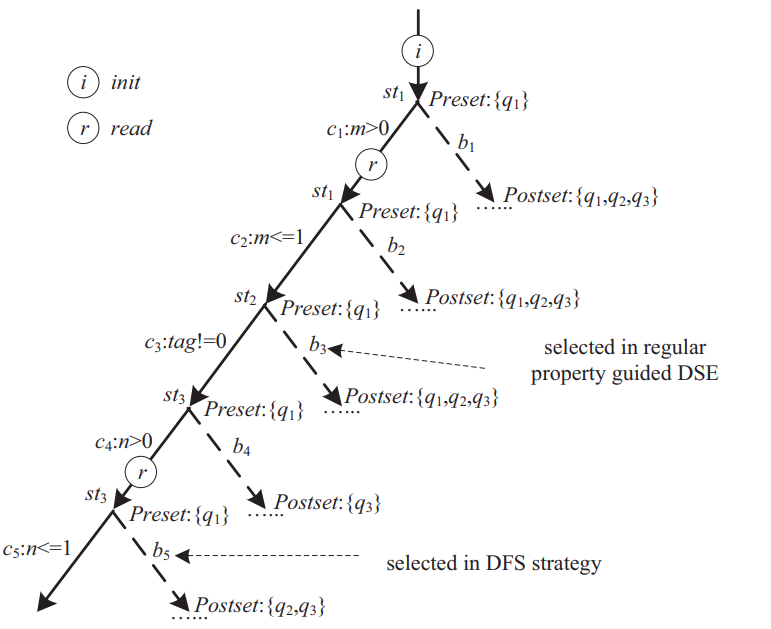
\includegraphics{figures/dse.png}
				}
				%\includegraphics[scale=1.0]{figurefile}
				\caption{DSE}
				\label{fig:dse}
			\end{figure}
		\end{column}%
	\end{columns}
\end{frame}

\begin{frame}{What is KLEE}
	What is KLEE?
	\begin{itemize}
		\item<0-> KLEE is a dynamic symbolic execution engine built on top of the LLVM compiler infrastructure
		\item<0-> KLEE can also be used as a bug finding tool
	\end{itemize}
\end{frame}

\subsection{Main Contributions}
\begin{frame}{Contributions}
	This paper makes two contributions.
	\begin{enumerate}
		\item<0-> It presents a new symbolic execution tool, KLEE, which they designed for robust,
		      deep checking of a broad range of applications, leveraging several years of lessons from their
		      previous tool, EXE
		\item<0-> It shows that KLEE’s automatically-generated tests get high coverage on a diverse set of real,
		      complicated, and environmentally-intensive programs.
	\end{enumerate}
\end{frame}

\begin{frame}{KLEE’s preformance}
	\begin{block}<1->{KLEE's preformance}
		\begin{itemize}
			\item<1->  KLEE gets high coverage on a broad set of complex programs.
			\item<1->  KLEE can get significantly more code coverage than a concentrated, sustained manual effort.
			\item<1->  With one exception, KLEE achieved these highcoverage results on unaltered applications.
			\item<1->  KLEE finds important errors in heavily-tested code.
			\item<1->  The fact that KLEE test cases can be run on the raw version of the code (e.g., compiled with gcc) greatly
			      simplifies debugging and error reporting.
			\item<1->  When used to crosscheck purportedly identical BUSYBOX and GNU COREUTILS tools,
			      it automatically found functional correctness errors and a myriad of inconsistencies.
			\item<1->  KLEE can also be applied to non-application code.
		\end{itemize}
	\end{block}
\end{frame}

\subsection{KLEE Overivew}
\begin{frame}{Basic Architecture}
	\begin{itemize}
		\item <0-> The core of KLEE is an interpreter loop which selects a state to run and then symbolically executes a
		      single instruction in the context of that state.
		\item <0-> Storage locations for a state — registers, stack and heap objects — refer to \textbf{expressions} (trees) instead of raw data values.
		\item <0-> The \textbf{leaves} of an expression are \textbf{symbolic variables or constants}, and
		      the \textbf{interior nodes} come from \textbf{LLVM assembly language operations}.
	\end{itemize}
\end{frame}

\begin{frame}{Basic Architecture}
	\begin{itemize}
		\item <0-> \textbf{Conditional branches} take a boolean expression
		      (branch condition) and alter the instruction pointer of
		      the state based on whether the condition is true or false.
		\item <0-> \textbf{Potentially dangerous operations} implicitly generate
		      branches that check if any input value exists that could
		      cause an error.
		\item <0-> \textbf{Load and store instructions} generate checks: in this case to check that the
		      address is in-bounds of a valid memory object
		\item <0-> \textbf{If a pointer can refer to many objects}, when a dereferenced pointer p
		      can refer to N objects, KLEE clones the current state N times.
	\end{itemize}
\end{frame}



\section{Code Review}
\subsection{Overview}
\begin{frame}{Overview}
	This is the general struct of KLEE
	\begin{figure}[!t]
		\centering
		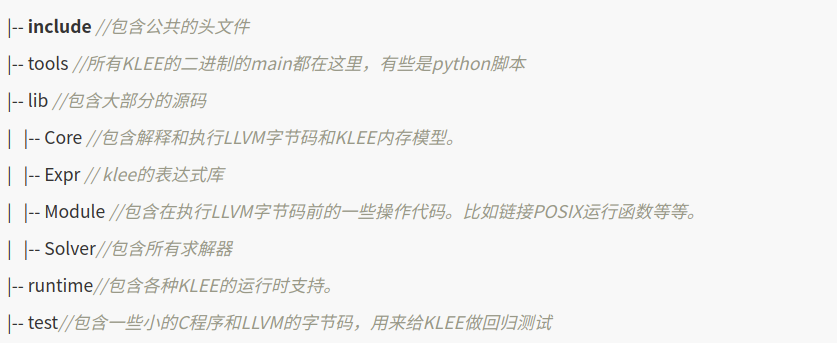
\includegraphics[width=\textwidth]{figures/code_struct.png}
		\caption{General Struct}
		\label{fig:klee_overview}
	\end{figure}
\end{frame}

\subsection{Main Execution Flow}
\begin{frame}[fragile]
	\frametitle{Main Execution Flow}
	% \begin{minted}[fontsize=\footnotesize\rmfamily, breaklines=true, tabsize=4, linenos, breaklines=true, frame=lines]{cpp}
	% \end{minted}
	\begin{columns}[T]
		\begin{column}<0->{0.5\textwidth}
			This is the main flow of execution of KLEE, source code can be seen at \verb|lib/Core/Executor.cpp:2954|\\
			Searcher->selectState selects a state and returns to the variable \textit{state},
			then function \textit{stepInstruction} points pc (program counter) to instruction to be executed.
			After this, function \textit{executeInstruction} executes this Instruction according to its type.
		\end{column}
		\hfill
		\begin{column}<0->{0.5\textwidth}
			\begin{lstlisting}
while (!states.empty() && !haltExecution) {
  ExecutionState &state = searcher->selectState();
  KInstruction *ki = state.pc;
  stepInstruction(state);

  executeInstruction(state, ki);
  timers.invoke();
  if (::dumpStates) dumpStates();
  if (::dumpPTree) dumpPTree();

  checkMemoryUsage();

  updateStates(&state);
}
    \end{lstlisting}
		\end{column}
	\end{columns}
\end{frame}

\subsection{Implementaion of some important feature}
\begin{frame}[fragile]
	\frametitle{Branch (Br)}
	\begin{columns}[T]
		\begin{column}<0->{0.4\textwidth}
			Br Instruction has to types: unconditional branch (function as goto in C) and conditional branch.

			In unconditional case, all we have to do is to transfer BasicBlock from current BasicBlock
			to its successor.
		\end{column}
		\hfill
		\begin{column}<0->{0.6\textwidth}
			\begin{lstlisting}
case Instruction::Br: {
  BranchInst *bi = cast<BranchInst>(i);
  if (bi->isUnconditional()) {
    transferToBasicBlock(bi->getSuccessor(0), bi->getParent(), state);
  } 
      \end{lstlisting}
		\end{column}
	\end{columns}
\end{frame}

\begin{frame}[fragile]
	\frametitle{Branch (Br)}
	In conditional case, we will\\
	\begin{itemize}
		\only<1> {\item fork the current state and add corresponding condition to the constraint set.\\}
		      \only<2> {\item send the constraint sets to solver (STP, Z3 etc.) to determine if the
		      branch condition is either provably true (return trueState) or provably false (return falseState).}
		      \only<3> {\item check if both branches are all provably true, and transfer the BasicBlocks by function transferToBasicBlock }
	\end{itemize}

	\begin{lstlisting}[firstnumber=3]
case Instruction::Br: {
  /* ... */
  } else {
    assert(bi->getCondition() == bi->getOperand(0) && "Wrong operand index!");
    ref<Expr> cond = eval(ki, 0, state).value;

    cond = optimizer.optimizeExpr(cond, false);
    Executor::StatePair branches = fork(state, cond, false);

    if (statsTracker && state.stack.back().kf->trackCoverage)
      statsTracker->markBranchVisited(branches.first, branches.second);

    if (branches.first)
      transferToBasicBlock(bi->getSuccessor(0), bi->getParent(), *branches.first);
    if (branches.second)
      transferToBasicBlock(bi->getSuccessor(1), bi->getParent(), *branches.second);
  }
  break;
}
  \end{lstlisting}
\end{frame}

\begin{frame}[fragile]
	\frametitle{Zero division check}

	Instrument function \verb|klee_div_zero_check| before instructions like \verb|sdiv| when the divisor of the instruction is 0.

	\begin{lstlisting}
void klee_div_zero_check(long long z) {
  if (z == 0)
    klee_report_error(__FILE__, __LINE__, "divide by zero", "div.err");
}
  \end{lstlisting}
	\begin{lstlisting}
  LLVMContext &ctx = M.getContext();
  KleeIRMetaData md(ctx);
  auto divZeroCheckFunction = M.getOrInsertFunction("klee_div_zero_check", Type::getVoidTy(ctx), Type::getInt64Ty(ctx) KLEE_LLVM_GOIF_TERMINATOR);

  for (auto &divInst : divInstruction) {
    llvm::IRBuilder<> Builder(divInst /* Inserts before divInst*/);
    auto denominator = Builder.CreateIntCast(divInst->getOperand(1), Type::getInt64Ty(ctx),
                              false, "int_cast_to_i64");
    Builder.CreateCall(divZeroCheckFunction, denominator);
    md.addAnnotation(*divInst, "klee.check.div", "True");
  \end{lstlisting}
\end{frame}

\begin{frame}[fragile]
	\frametitle{Boundary check}
	\begin{columns}[T]
		\begin{column}<0->{0.4\textwidth}
			When encountering an array operation instruction such as Store, Load, etc., klee will check the array boundary overflow
		\end{column}
		\hfill
		\begin{column}<0->{0.6\textwidth}
			\begin{lstlisting}
ref<Expr> getBoundsCheckOffset(ref<Expr> offset, unsigned bytes) const {
  if (bytes<=size) {
    return UltExpr::create(offset, ConstantExpr::alloc(size - bytes + 1, Context::get().getPointerWidth()));
  } else {
    return ConstantExpr::alloc(0, Expr::Bool);
  }
}
      \end{lstlisting}
		\end{column}
	\end{columns}


\end{frame}

\subsection{State Scheduling}
\begin{frame}[fragile]{Scheduling}
	\begin{lstlisting}
Searcher *getNewSearcher(Searcher::CoreSearchType type, Executor &executor) {
  Searcher *searcher = NULL;
  switch (type) {
  case Searcher::DFS: searcher = new DFSSearcher(); break;
  case Searcher::BFS: searcher = new BFSSearcher(); break;
  case Searcher::RandomState: searcher = new RandomSearcher(); break;
  case Searcher::RandomPath: searcher = new RandomPathSearcher(executor); break;
  case Searcher::NURS_CovNew: searcher = new WeightedRandomSearcher(WeightedRandomSearcher::CoveringNew); break;
  case Searcher::NURS_MD2U: searcher = new WeightedRandomSearcher(WeightedRandomSearcher::MinDistToUncovered); break;
  case Searcher::NURS_Depth: searcher = new WeightedRandomSearcher(WeightedRandomSearcher::Depth); break;
  case Searcher::NURS_RP: searcher = new WeightedRandomSearcher(WeightedRandomSearcher::RP); break;
  case Searcher::NURS_ICnt: searcher = new WeightedRandomSearcher(WeightedRandomSearcher::InstCount); break;
  case Searcher::NURS_CPICnt: searcher = new WeightedRandomSearcher(WeightedRandomSearcher::CPInstCount); break;
  case Searcher::NURS_QC: searcher = new WeightedRandomSearcher(WeightedRandomSearcher::QueryCost); break;
  }

  return searcher;
}
  \end{lstlisting}
\end{frame}

\begin{frame}[fragile]{Random Path Selection}
	\begin{columns}[T]
		\begin{column}<0->{0.4\textwidth}
			States are selected by traversing this tree from the root and randomly
			selecting the path to follow at branch points. Therefore,
			when a branch point is reached, the set of states in each
			subtree has equal probability of being selected, regardless of the size of their subtrees.
		\end{column}
		\hfill
		\begin{column}<0->{0.6\textwidth}
			\begin{lstlisting}
ExecutionState &RandomPathSearcher::selectState() {
  unsigned flips=0, bits=0;
  PTreeNode *n = executor.processTree->root.get();
  while (!n->state) {
    if (!n->left) {
      n = n->right.get();
    } else if (!n->right) {
      n = n->left.get();
    } else {
      if (bits==0) {
        flips = theRNG.getInt32();
        bits = 32;
      }
      --bits;
      n = (flips&(1<<bits)) ? n->left.get() : n->right.get();
    }
  }

  return *n->state;
}
      \end{lstlisting}
		\end{column}
	\end{columns}
\end{frame}


\begin{frame}[fragile]{Coverage-Optimized Search}
	All kinds of searcher are implemented in \verb|lib/Core/Searcher.cpp|. Below is
	the implementation of the Coverage-Optimized Search.\\
	% RNG is the abbreviation of random number generator, and class \verb|RNG| is implemented in 
	% \verb|include/klee/Internal/ADT/RNG.h| . When \verb|CoreSearcherType| is \verb|NURS_CovNew|, which means
	% Non Uniform Random Search (NURS) with Coverage-New, function \verb|WeightedRandomSearcher::selectState| 
	% is called.
	States are preserved in a Red-Black tree, and its weight is computed according to the \verb|type| attribute of
	the  \verb|state|. After a new state is generated, it's inserted in the RB Tree (namely DiscretePDF). After a state
	is selected (In Coverage-Optimized Search, it's randomly selected as well), the node is removed from the RB-Tree.
	\newline

	\begin{lstlisting}[frame=lines]
ExecutionState &WeightedRandomSearcher::selectState() {
  return *states->choose(theRNG.getDoubleL());
}
  \end{lstlisting}
	% \caption{lib/Core/Searcher.cpp:192}
\end{frame}
\begin{frame}[fragile]{Coverage-Optimized Search}
	\begin{columns}[T]
		\begin{column}<0->{0.5\textwidth}
			\begin{lstlisting}[numbersep=4pt]
double WeightedRandomSearcher::getWeight(ExecutionState *es) {
  switch(type) {
  default:
  case Depth:
    return es->depth;
  case RP:
    return std::pow(0.5, es->depth);
  case InstCount: {
    uint64_t count = theStatisticManager->getIndexedValue(stats::instructions, es->pc->info->id);
    double inv = 1. / std::max((uint64_t) 1, count);
    return inv * inv;
  }
  case CPInstCount: {
    StackFrame &sf = es->stack.back();
    uint64_t count = sf.callPathNode->statistics.getValue(stats::instructions);
    double inv = 1. / std::max((uint64_t) 1, count);
    return inv;
  }
        \end{lstlisting}
		\end{column}
		\hfill
		\begin{column}<0->{0.5\textwidth}
			\begin{lstlisting}[firstnumber=last,numbersep=4pt]
    case QueryCost:
    return (es->queryCost.toSeconds() < .1) ? 1. : 1./ es->queryCost.toSeconds();
  case CoveringNew:
  case MinDistToUncovered: {
    uint64_t md2u = computeMinDistToUncovered(es->pc, es->stack.back().minDistToUncoveredOnReturn);
    double invMD2U = 1. / (md2u ? md2u : 10000);
    if (type==CoveringNew) {
      double invCovNew = 0.;
      if (es->instsSinceCovNew)
        invCovNew = 1. / std::max(1, (int) es->instsSinceCovNew - 1000);
      return (invCovNew * invCovNew + invMD2U * invMD2U);
    } else {
      return invMD2U * invMD2U;
    }
  }
  }
}
    \end{lstlisting}
		\end{column}
	\end{columns}
\end{frame}


\subsection{Memory Organization}

\begin{frame}[fragile]{Memory Organization}
	\begin{columns}[T]
		\begin{column}<0->{0.4\textwidth}
			Use Alloca as an example.
			When instruction type is \verb|alloca|, in function \verb|executeInstruction| it turns to the \textit{Alloca} case.
			In this case, a pointer is generated accroding to the size of the element. Then \verb|executeAlloc| is called.
		\end{column}
		\hfill
		\begin{column}<0->{0.6\textwidth}
			\begin{lstlisting}
case Instruction::Alloca: {
  AllocaInst *ai = cast<AllocaInst>(i);
  // KModule: 基于 llvm::module, 但添加了其他 klee 相关信息
  unsigned elementSize =  
    kmodule->targetData->getTypeStoreSize(ai->getAllocatedType());
  // 根据上面拿到的元素大小创建一个指针
  ref<Expr> size = Expr::createPointer(elementSize);
  if (ai->isArrayAllocation()) {
    ref<Expr> count = eval(ki, 0, state).value;
    count = Expr::createZExtToPointerWidth(count);
    size = MulExpr::create(size, count);
  }
  executeAlloc(state, size, true, ki);
  break;
}
      \end{lstlisting}
		\end{column}
	\end{columns}
\end{frame}


\begin{frame}{Memory Organization}
	MemoryObject's represent allocation sites in the program (calls to malloc, stack objects, global variables) and,
	at least conceptually, can be thought of as the unique name for the object allocated at that site.
	ObjectState's are used to store the actual contents of a MemoryObject in a particular ExecutionState (but can be shared).
\end{frame}
\begin{frame}[fragile]{Memory Organization}
	\begin{lstlisting}
size = toUnique(state, size);
if (ConstantExpr *CE = dyn_cast<ConstantExpr>(size)) {
  const llvm::Value *allocSite = state.prevPC->inst;
  if (allocationAlignment == 0) {
    allocationAlignment = getAllocationAlignment(allocSite);
  }
  MemoryObject *mo =
      memory->allocate(CE->getZExtValue(), isLocal, /*isGlobal=*/false, allocSite, allocationAlignment);
  if (!mo) {
    bindLocal(target, state, 
              ConstantExpr::alloc(0, Context::get().getPointerWidth()));
  } else {
    ObjectState *os = bindObjectInState(state, mo, isLocal);
    if (zeroMemory) os->initializeToZero();
    else os->initializeToRandom();
    bindLocal(target, state, mo->getBaseExpr());
    
    if (reallocFrom) {
      unsigned count = std::min(reallocFrom->size, os->size);
      for (unsigned i=0; i<count; i++)
        os->write(i, reallocFrom->read8(i));
      state.addressSpace.unbindObject(reallocFrom->getObject());
    }
  }
}
      \end{lstlisting}
\end{frame}

\begin{frame}[fragile]{Memory Organization}
	\begin{columns}[T]
		\begin{column}<0->{0.6\textwidth}
			Each ExecutionState stores a mapping of MemoryObjects -> ObjectState using the AddressSpace data structure
			(implemented as an immutable tree so that copying is cheap and the shared structure is exploited).
			Each AddressSpace may "own" some subset of the ObjectStates in the mapping.
			When an AddressSpace is duplicated it loses ownership of the ObjectState in the map.
			Any subsequent write to an ObjectState will create a copy of the object (AddressSpace::getWriteable).
			This is the COW mechanism (which gets used for all objects, not just globals).
		\end{column}
		\hfill
		\begin{column}<0->{0.4\textwidth}
			\begin{lstlisting}
ObjectState *Executor::bindObjectInState(ExecutionState &state, const MemoryObject *mo, bool isLocal, const Array *array) {
  ObjectState *os = array ? new ObjectState(mo, array) : new ObjectState(mo);
  state.addressSpace.bindObject(mo, os);

  if (isLocal)
    state.stack.back().allocas.push_back(mo);

  return os;
}
      \end{lstlisting}
		\end{column}
	\end{columns}
\end{frame}
\begin{frame}{Memory Organization}
	From the point of view of the state and this mapping there is no distinction between stack, heap,
	and global objects. The only special handling for stack objects is that the MemoryObject is marked
	as isLocal and the MemoryObject is stored in the StackFrame alloca list. When the StackFrame is popped
	these objects are then unbound so that the state can no longer access the memory directly
	(references to the memory object may still remain in ReadExprs, but conceptually the actual memory is no longer addressable).
\end{frame}



\subsection{Query Optimization}

\begin{frame}{Constraint independence}
	\textbf{Constraint independence} divides constraint sets into disjoint independent subsets.
	By explicitly tracking these subsets, KLEE can frequently eliminate irrelevant constraints

	For example, given the constraint set ${i < j, j < 20, k > 0}$, a query of whether $i = 20$
	just requires the first two constraints.
\end{frame}

\begin{frame}[fragile]{Constraint independence}
	\begin{lstlisting}
IndependentElementSet getIndependentConstraints(const Query& query,
                        std::vector< ref<Expr> > &result) {
  IndependentElementSet eltsClosure(query.expr);
  std::vector< std::pair<ref<Expr>, IndependentElementSet> > worklist;
  for (const auto &constraint : query.constraints)
  worklist.push_back(std::make_pair(constraint, IndependentElementSet(constraint)));
  bool done = false;
  do {
    done = true;
    std::vector< std::pair<ref<Expr>, IndependentElementSet> > newWorklist;
    for (std::vector< std::pair<ref<Expr>, IndependentElementSet> >::iterator
    it = worklist.begin(), ie = worklist.end(); it != ie; ++it) {
        if (it->second.intersects(eltsClosure)) {
            if (eltsClosure.add(it->second))
            done = false;
            result.push_back(it->first);
          } else {
            newWorklist.push_back(*it);
          }
      }
    worklist.swap(newWorklist);
  } while (!done);
  return eltsClosure;
}
  \end{lstlisting}
\end{frame}

\begin{frame}{Constraint Set Simplification}
	\textbf{Constraint Set Simplification} : klee simplifies the constraint set by rewriting previous
	constraints when new equality constraints are added to the
	constraint set. The constraint $x <10$. followed by $x=5$, substituting the value for
	x into the first constraint simplifies it to true, which KLEE eliminates.
\end{frame}

\begin{frame}[fragile]{Constraint Set Simplification}
	\begin{lstlisting}
ref<Expr> ConstraintManager::simplifyExpr(const ConstraintSet &constraints,
                      const ref<Expr> &e) {
  if (isa<ConstantExpr>(e))
    return e;
  std::map< ref<Expr>, ref<Expr> > equalities;
  for (auto &constraint : constraints) {
      if (const EqExpr *ee = dyn_cast<EqExpr>(constraint)) {
          if (isa<ConstantExpr>(ee->left)) {
              equalities.insert(std::make_pair(ee->right,ee->left));
              } else {
                equalities.insert(
                std::make_pair(constraint, ConstantExpr::alloc(1, Expr::Bool)));
              }
      } else {
          equalities.insert(
          std::make_pair(constraint, ConstantExpr::alloc(1, Expr::Bool)));
      }
  }

  return ExprReplaceVisitor2(equalities).visit(e);
}
      \end{lstlisting}
\end{frame}

\begin{frame}[fragile]{Expression Rewriting}
	\begin{columns}[T]
		\begin{column}<0->{0.4\textwidth}
			\textbf{Expression Rewriting}: simple arithmetic sim-
			plifications $(x + 0 = x)$, strength reduction $(x * 2^n
				= x << n)$, linear simplification $(2*x - x = x)$.
		\end{column}
		\hfill
		\begin{column}<0->{0.7\textwidth}
			\begin{lstlisting}
bool ConstraintManager::rewriteConstraints(ExprVisitor &visitor) {
  ConstraintSet old;
  bool changed = false;

  std::swap(constraints, old);
  for (auto &ce : old) {
      ref<Expr> e = visitor.visit(ce);

      if (e!=ce) {
          addConstraintInternal(e); // enable further reductions
          changed = true;
        } else {
          constraints.push_back(ce);
        }
    }

  return changed;
}
      \end{lstlisting}
		\end{column}
	\end{columns}
\end{frame}

\begin{frame}[fragile]{Counter-example Cache}

	Redundant queries are frequent, and a simple cache is effective at eliminating a
	large number of them.The counter-example cache maps sets of constraints to counter-examples (i.e., variable assignments), along with a special sentinel used when a set
	of constraints has no solution.
	\begin{itemize}
		\item<0-> When a subset of a constraint set has no solution,
		      then neither does the original constraint set.
		\item<0-> When a superset of a constraint set has a solution,
		      that solution also satisfies the original constraint set.
		\item<0-> When a subset of a constraint set has a solution, it is
		      likely that this is also a solution for the original set.
	\end{itemize}
\end{frame}

\begin{frame}[fragile]{Counter-example Cache}
	\begin{columns}[T]
		\begin{column}<0->{0.5\textwidth}
			\begin{lstlisting}[numbersep=4pt]
bool CexCachingSolver::searchForAssignment(KeyType &key, Assignment *&result) {
    Assignment * const *lookup = cache.lookup(key);
    if (lookup) {
        result = *lookup;
        return true;
      }
    if (CexCacheTryAll) {
        // Look for a satisfying assignment for a superset, which is trivially an
        // assignment for any subset.
        Assignment **lookup = 0;
        if (CexCacheSuperSet)
        lookup = cache.findSuperset(key, NonNullAssignment());
        if (!lookup)
        lookup = cache.findSubset(key, NullAssignment());
        // If either lookup succeeded, then we have a cached solution.
        if (lookup) {
            result = *lookup;
            return true;
          }
          \end{lstlisting}
		\end{column}
		\hfill
		\begin{column}<0->{0.5\textwidth}
			\begin{lstlisting}[firstnumber=last,numbersep=4pt]
// Otherwise, iterate through the set of current assignments to see if one
// of them satisfies the query.
        for (assignmentsTable_ty::iterator it = assignmentsTable.begin(),
        ie = assignmentsTable.end(); it != ie; ++it) {
            Assignment *a = *it;
            if (a->satisfies(key.begin(), key.end())) {
                result = a;
                return true;
              }
          }
      } 
    return false;
  }
      \end{lstlisting}
		\end{column}
	\end{columns}
\end{frame}

\subsection{Solver}
\begin{frame}[fragile]{Solver}
	\begin{columns}[T]
		\begin{column}<0->{0.3\textwidth}
			When encountering conditional Br instructions or supposed errors, a solver (STP, Z3, etc.) is called.
		\end{column}
		\hfill
		\begin{column}<0->{0.7\textwidth}
			\begin{lstlisting}
bool CexCachingSolver::getAssignment(const Query& query, Assignment *&result) {
  KeyType key;
  if (lookupAssignment(query, key, result))
    return true;

  std::vector<const Array*> objects;
  findSymbolicObjects(key.begin(), key.end(), objects);

  std::vector< std::vector<unsigned char> > values;
  bool hasSolution;
  if (!solver->impl->computeInitialValues(query, objects, values, hasSolution))
    return false;
    
  /* ...*/
  
  result = binding;
  cache.insert(key, binding);

  return true;
}
    \end{lstlisting}
		\end{column}
	\end{columns}
\end{frame}
\begin{frame}
	\frametitle{Call stack of solver}
	\begin{center}
		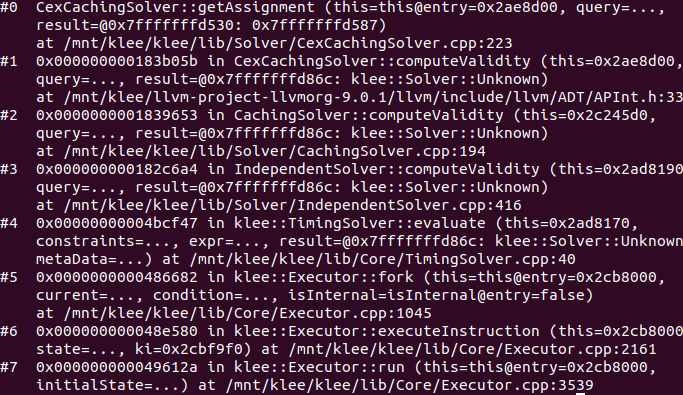
\includegraphics[width=\textwidth]{figures/STPSolverCallStack.png}
	\end{center}
\end{frame}

\subsection{Environment Modeling}
\begin{frame}{Environment Modeling}
	Handle the environment by redirecting calls that access it to models that understand the 
  semantics of the desired action well enough to generate the required constraints,
  these models are written in normal C code,2,500 lines of code to
	define simple models for roughly 40 system calls
	\\ ALL shared libraries are initialized by $\_\_uClibc\_main$
\end{frame}

\begin{frame}[fragile]{Environment Modeling}
	\begin{columns}[T]
		\begin{column}<0->{0.5\textwidth}
			\begin{lstlisting}[numbersep=4pt]
int main(int argc, char **argv, char **envp) {
  switch (Libc) {
    case LibcType::UcLibc:
    linkWithUclibc(LibraryDir, opt_suffix, loadedModules);
    break;
}
linkWithUclibc(StringRef libDir, std::string opt_suffix,
    std::vector<std::unique_ptr<llvm::Module>> &modules) {
  for (auto i = newModules, j = modules.size(); i < j; ++i) {
    replaceOrRenameFunction(modules[i].get(), "__libc_open", "open");
    replaceOrRenameFunction(modules[i].get(), "__libc_fcntl", "fcntl");
  }
  createLibCWrapper(modules, EntryPoint, "__uClibc_main");
    } /* ... */
      \end{lstlisting}
		\end{column}
		\hfill
		\begin{column}<0->{0.5\textwidth}
			\begin{lstlisting}[firstnumber=last, numbersep=4pt]
createLibCWrapper(std::vector<std::unique_ptr<llvm::Module>> &modules, llvm::StringRef intendedFunction, llvm::StringRef libcMainFunction) {
  llvm::Function *libcMainFn = nullptr;
  for (auto &module : modules) {
    if ((libcMainFn = module->getFunction(libcMainFunction)))
      break;
  }
  /* ... */
  BasicBlock *bb = BasicBlock::Create(ctx, "entry", stub);
  llvm::IRBuilder<> Builder(bb);  
  /* ... */ 
  Builder.CreateCall(libcMainFn, args);
  Builder.CreateUnreachable();
}
      \end{lstlisting}
		\end{column}
	\end{columns}
\end{frame}

\begin{frame}[fragile]{Environment Modeling}
	\begin{columns}[T]
		\begin{column}<0->{0.4\textwidth}
			For each file system operation we check if the action is
			for an actual concrete file on disk or a symbolic file. For
			concrete files, we simply invoke the corresponding system
			call in the running operating system. For symbolic
			files we emulate the operation’s effect on a simple sym-
			bolic file system, private to each state.
		\end{column}
		\hfill
		\begin{column}<0->{0.6\textwidth}
			\begin{lstlisting}
ssize_t read(int fd, void *buf, size_t count) {
  if (is_invalid(fd)) {
    errno = EBADF;
    return -1;
  }
  struct klee_fd *f = &fds[fd];
  if (is_concrete_file(f)) {
    int r = pread(f->real_fd, buf, count, f->off);
    if (r != -1)
      f->off += r;
    return r;
  } else {
    /* sym files are fixed size: don’t read beyond the end. */
    if (f->off >= f->size)
      return 0;
    count = min(count, f->size - f->off);
    memcpy(buf, f->file data + f->off, count);  
    f->off += count;
    return count;
  }
 }
      \end{lstlisting}
		\end{column}
	\end{columns}
\end{frame}

% \begin{algorithm}[H]
% 	\caption{HOSVD}
% 	\small 
% 	\KwIn{HOSVD($\mathcal{X},R_{1},R_{2}.....R_{N}$) }
% 	\KwOut{ $\mathcal{G},A_{(1)},A_{(2)}......A_{(N)} $ }
	
% 	\For{$k=1$ to $N$ }
% 	{
% 		$A_{(n)}\leftarrow R_{n}$left singular matrix of $X_{(n)}$
% 	}
% 	$\mathcal{G}=\leftarrow \mathcal{X} \times A_{(1)}^{T} \times A_{(2)}^{T}...... \times A_{(N)}^{T}$\\
% 	\Return $\mathcal{G},A_{(1)},A_{(2)}......A_{(N)} $
% \end{algorithm}

\section{KLEE Usage}
\subsection{Command line options}
\begin{frame}[fragile]{Command line options}
  \begin{enumerate}
    \item<0-> Compling to LLVM bitcode: \verb|clang -I ../../include -emit-llvm -c -g -O0 -Xclang -disable-O0-optnone pragram.c|
    \item<0-> General usage of KLEE: \verb|klee [klee-options] <program.bc> [program-options]|
    \item<0-> Set main search heuristics: \verb|klee --search=random-state --search=nurs:md2u program.o| % round-robin fashion
  \end{enumerate}
  Other options can be seen at \href{https://klee.github.io/docs/options/}{https://klee.github.io/docs/options/}
\end{frame}

% \subsection{gdb debugging demo}


\section{The End}
\begin{frame}{Thank you}
	\begin{center}
		\begin{minipage}{1\textwidth}
			\setbeamercolor{mybox}{fg=white, bg=black!50!blue}
			\begin{beamercolorbox}[wd=0.70\textwidth, rounded=true, shadow=true]{mybox}
				\LARGE \centering Thank you for listening!  %结束语
			\end{beamercolorbox}
		\end{minipage}
	\end{center}
\end{frame}

\begin{frame}{Q\&A}
	\begin{center}
		\begin{minipage}{1\textwidth}
			\setbeamercolor{mybox}{fg=white, bg=black!50!blue}
			\begin{beamercolorbox}[wd=0.70\textwidth, rounded=true, shadow=true]{mybox}
				\LARGE \centering  Questions?  %请求提问
			\end{beamercolorbox}
		\end{minipage}
	\end{center}
\end{frame}

% -----------------------------------------------------------------------------
\end{document}
%文档结束